%\PassOptionsToPackage{landscape}{geometry}
\documentclass[aspectratio=169]{beamer}

%\usepackage{bm}

\usepackage{xcolor}
\usepackage{colortbl}
\def\boldred#1{\color{red}\textbf{#1}}

\def\IC{\mathbb{C}}
\def\IF{\mathbb{F}}
\def\II{\mathbb{I}}
\def\IM{\mathbb{M}}
\def\IN{\mathbb{N}}
\def\IP{\mathbb{P}}
\def\IR{\mathbb{R}}
\def\IZ{\mathbb{Z}}

\def\ba{\mathbf{a}}
\def\bb{\mathbf{b}}
\def\bc{\mathbf{c}}
\def\be{\mathbf{e}}
\def\bh{\mathbf{h}}
\def\bi{\mathbf{i}}
\def\bj{\mathbf{j}}
\def\bk{\mathbf{k}}
\def\bn{\mathbf{n}}
\def\bp{\mathbf{p}}
\def\br{\mathbf{r}}
\def\bs{\mathbf{s}}
\def\bu{\mathbf{u}}
\def\bv{\mathbf{v}}
\def\bw{\mathbf{w}}
\def\bx{\mathbf{x}}
\def\by{\mathbf{y}}
\def\bz{\mathbf{z}}

\def\bB{\mathbf{B}}
\def\bD{\mathbf{D}}
\def\bF{\mathbf{F}}
\def\bG{\mathbf{G}}
\def\bN{\mathbf{N}}
\def\bR{\mathbf{R}}
\def\bS{\mathbf{S}}
\def\bT{\mathbf{T}}
\def\b0{\mathbf{0}}

\bmdefine{\bmu}{\bm{\mu}}

\def\A{\mathcal{A}}
\def\B{\mathcal{B}}
\def\C{\mathcal{C}}
\def\D{\mathcal{D}}
\def\E{\mathcal{E}}
\def\F{\mathcal{F}}
\def\G{\mathcal{G}}
\def\I{\mathcal{I}}
\def\L{\mathcal{L}}
\def\M{\mathcal{M}}
\def\N{\mathcal{N}}
\def\P{\mathcal{P}}
\def\R{\mathcal{R}}
\def\S{\mathcal{S}}
\def\T{\mathcal{T}}
\def\U{\mathcal{U}}
\def\V{\mathcal{V}}

\def\nbOne{{\mathchoice {\rm 1\mskip-4mu l} {\rm 1\mskip-4mu l}
{\rm 1\mskip-4.5mu l} {\rm 1\mskip-5mu l}}}

\def\cov{\ensuremath{\mathsf{cov}}}
\def\Var{\ensuremath{\mathsf{Var}\ }}

\newtheorem{proposition}[theorem]{Proposition}
\newtheorem{property}[theorem]{Property}
\newtheorem{importantproperty}[theorem]{Property}
\newtheorem{importanttheorem}[theorem]{Theorem}
%\newtheorem{lemma}[theorem]{Lemma}



\setbeamertemplate{navigation symbols}{}
\setbeamertemplate{footline}
{%
	\quad\insertsection\hfill p. \insertpagenumber\quad\mbox{}\vskip2pt
}
\usecolortheme{orchid}
\setbeamertemplate{theorems}[numbered]

\makeatletter
\newlength\beamerleftmargin
\setlength\beamerleftmargin{\Gm@lmargin}
\makeatother

%%%%%%% 
%% Definitions in yellow boxes
\usepackage{etoolbox}
\setbeamercolor{block title}{use=structure,fg=structure.fg,bg=structure.fg!05!bg}
\setbeamercolor{block body}{parent=normal text,use=block title,bg=block title.bg!20!bg}

\BeforeBeginEnvironment{definition}{%
	\setbeamercolor{block title}{fg=black,bg=yellow!20!white}
	\setbeamercolor{block body}{fg=black, bg=yellow!05!white}
}
\AfterEndEnvironment{definition}{
	\setbeamercolor{block title}{use=structure,fg=structure.fg,bg=structure.fg!20!bg}
	\setbeamercolor{block body}{parent=normal text,use=block title,bg=block title.bg!50!bg, fg=black}
}
\BeforeBeginEnvironment{importanttheorem}{%
	\setbeamercolor{block title}{fg=black,bg=red!20!white}
	\setbeamercolor{block body}{fg=black, bg=red!05!white}
}
\AfterEndEnvironment{importanttheorem}{
	\setbeamercolor{block title}{use=structure,fg=structure.fg,bg=structure.fg!20!bg}
	\setbeamercolor{block body}{parent=normal text,use=block title,bg=block title.bg!50!bg, fg=black}
}
\BeforeBeginEnvironment{importantproperty}{%
	\setbeamercolor{block title}{fg=black,bg=red!50!white}
	\setbeamercolor{block body}{fg=black, bg=red!30!white}
}
\AfterEndEnvironment{importantproperty}{
	\setbeamercolor{block title}{use=structure,fg=structure.fg,bg=structure.fg!20!bg}
	\setbeamercolor{block body}{parent=normal text,use=block title,bg=block title.bg!50!bg, fg=black}
}


%%%%%%%%%%%%%%%%%
\usepackage{tikz}
\usetikzlibrary{shapes,arrows}
\usetikzlibrary{positioning}
\tikzstyle{cloud} = [draw, ellipse,fill=red!20, node distance=0.87cm,
minimum height=2em]
\tikzstyle{line} = [draw, -latex']
\usetikzlibrary{shapes.symbols,shapes.callouts,patterns}
\usetikzlibrary{calc,fit}
\usetikzlibrary{backgrounds}

\usetikzlibrary{decorations.pathmorphing,backgrounds,positioning,fit,petri}
\usetikzlibrary{automata}


% Beginning of a section
\AtBeginSection[]{
	{
		\setbeamercolor{background canvas}{bg=orange!10}
		\begin{frame}[noframenumbering,plain]
			\framesubtitle{\nameofthepart Chapter \insertromanpartnumber \ -- \iteminsert{\insertpart}}
			\tableofcontents[currentsection,currentsubsection]
		\end{frame}
	\addtocounter{page}{-1}
	%\addtocounter{framenumber}{-1} 
	}
}

\usepackage{bm}

%\usepackage{graphics}
\usepackage{graphicx}
\usepackage{amsmath,amssymb,amsthm}
\usepackage{bm}
%\usepackage{subfigure}

\usepackage{xcolor}
\usepackage{colortbl}

\def\boldred#1{\color{red}\textbf{#1}}

\def\IC{\mathbb{C}}
\def\IF{\mathbb{F}}
\def\II{\mathbb{I}}
\def\IM{\mathbb{M}}
\def\IN{\mathbb{N}}
\def\IP{\mathbb{P}}
\def\IR{\mathbb{R}}
\def\IZ{\mathbb{Z}}

\def\ba{\mathbf{a}}
\def\bb{\mathbf{b}}
\def\bc{\mathbf{c}}
\def\be{\mathbf{e}}
\def\bg{\mathbf{g}}
\def\bh{\mathbf{h}}
\def\bi{\mathbf{i}}
\def\bj{\mathbf{j}}
\def\bk{\mathbf{k}}
\def\bn{\mathbf{n}}
\def\bp{\mathbf{p}}
\def\br{\mathbf{r}}
\def\bs{\mathbf{s}}
\def\bu{\mathbf{u}}
\def\bv{\mathbf{v}}
\def\bw{\mathbf{w}}
\def\bx{\mathbf{x}}
\def\by{\mathbf{y}}
\def\bz{\mathbf{z}}

\def\bB{\mathbf{B}}
\def\bD{\mathbf{D}}
\def\bF{\mathbf{F}}
\def\bG{\mathbf{G}}
\def\bN{\mathbf{N}}
\def\bR{\mathbf{R}}
\def\bS{\mathbf{S}}
\def\bT{\mathbf{T}}
\def\b0{\mathbf{0}}

\bmdefine{\bmu}{\bm{\mu}}

\def\A{\mathcal{A}}
\def\B{\mathcal{B}}
\def\C{\mathcal{C}}
\def\D{\mathcal{D}}
\def\E{\mathcal{E}}
\def\F{\mathcal{F}}
\def\G{\mathcal{G}}
\def\I{\mathcal{I}}
\def\L{\mathcal{L}}
\def\M{\mathcal{M}}
\def\N{\mathcal{N}}
\def\P{\mathcal{P}}
\def\R{\mathcal{R}}
\def\S{\mathcal{S}}
\def\T{\mathcal{T}}
\def\U{\mathcal{U}}
\def\V{\mathcal{V}}

\def\nbOne{{\mathchoice {\rm 1\mskip-4mu l} {\rm 1\mskip-4mu l}
{\rm 1\mskip-4.5mu l} {\rm 1\mskip-5mu l}}}

\def\cov{\ensuremath{\mathsf{cov}}}
\def\Var{\ensuremath{\mathsf{Var}\ }}

\def\defword#1{\textbf{#1}\index{#1}}



%%%%%%%%%%%%%%%%%%%%%
%%%%%%%%%%%%%%%%%%%%%
%%
%%
%% NAVIGATION AND SECTIONING
%%
%%
%%%%%%%%%%%%%%%%%%%%%
%%%%%%%%%%%%%%%%%%%%%
\def\sgn{\ensuremath{\mathsf{sgn}}}

\newtheorem{proposition}[theorem]{Proposition}
\newtheorem{property}[theorem]{Property}
\newtheorem{importantproperty}[theorem]{Property}
\newtheorem{importanttheorem}[theorem]{Theorem}
%\newtheorem{lemma}[theorem]{Lemma}



\setbeamertemplate{navigation symbols}{}
\setbeamertemplate{footline}
{%
	\quad\insertsection\hfill p. \insertpagenumber\quad\mbox{}\vskip2pt
}
\usecolortheme{orchid}
\setbeamertemplate{theorems}[numbered]

\makeatletter
\newlength\beamerleftmargin
\setlength\beamerleftmargin{\Gm@lmargin}
\makeatother

%%%%%%%%%%%
% To have links to parts in the outline
\makeatletter
\AtBeginPart{%
	\addtocontents{toc}{\protect\beamer@partintoc{\the\c@part}{\beamer@partnameshort}{\the\c@page}}%
}
%% number, shortname, page.
\providecommand\beamer@partintoc[3]{%
	\ifnum\c@tocdepth=-1\relax
	% requesting onlyparts.
	\makebox[6em]{Chapter #1:} \textcolor{green!30!blue}{\hyperlink{#2}{#2}}
	\par
	\fi
}
\define@key{beamertoc}{onlyparts}[]{%
	\c@tocdepth=-1\relax
}
\makeatother%

\newcommand{\nameofthepart}{}
\newcommand{\nupart}[1]%
{   \part{#1}%
	\renewcommand{\nameofthepart}{#1}%
	{
		\setbeamercolor{background canvas}{bg=orange!50}
		\begin{frame}{#1}%\partpage 
			\hypertarget{\nameofthepart}{}\tableofcontents%
		\end{frame}
	}
}

% Beginning of a section
\AtBeginSection[]{
	{
		\setbeamercolor{background canvas}{bg=orange!10}
		\begin{frame}[noframenumbering,plain]
			\tableofcontents[currentsection,hideothersubsections]
		\end{frame}
		\addtocounter{page}{-1}
		%\addtocounter{framenumber}{-1} 
	}
}

% Beginning of a section
\AtBeginSubsection[]{
	{
		\setbeamercolor{background canvas}{bg=orange!10}
		\begin{frame}[noframenumbering,plain]
			\tableofcontents[sectionstyle=show/shaded,subsectionstyle=show/shaded/hide]
		\end{frame}
		\addtocounter{page}{-1}
		%\addtocounter{framenumber}{-1} 
	}
}




%%%%%%%%%%%%%%%%%%%%%
%%%%%%%%%%%%%%%%%%%%%
%%
%%
%% COLOURED ENVIRONMENTS
%%
%%
%%%%%%%%%%%%%%%%%%%%%
%%%%%%%%%%%%%%%%%%%%%
\newtheorem{proposition}[theorem]{Proposition}
\newtheorem{property}[theorem]{Property}
\newtheorem{importantproperty}[theorem]{Property}
\newtheorem{importanttheorem}[theorem]{Theorem}
%\newtheorem{lemma}[theorem]{Lemma}
%%%%%%% 
%% Definitions in yellow boxes
\usepackage{etoolbox}
\setbeamercolor{block title}{use=structure,fg=structure.fg,bg=structure.fg!05!bg}
\setbeamercolor{block body}{parent=normal text,use=block title,bg=block title.bg!20!bg}

\BeforeBeginEnvironment{definition}{%
	\setbeamercolor{block title}{fg=black,bg=yellow!20!white}
	\setbeamercolor{block body}{fg=black, bg=yellow!05!white}
}
\AfterEndEnvironment{definition}{
	\setbeamercolor{block title}{use=structure,fg=structure.fg,bg=structure.fg!20!bg}
	\setbeamercolor{block body}{parent=normal text,use=block title,bg=block title.bg!50!bg, fg=black}
}
\BeforeBeginEnvironment{importanttheorem}{%
	\setbeamercolor{block title}{fg=black,bg=red!20!white}
	\setbeamercolor{block body}{fg=black, bg=red!05!white}
}
\AfterEndEnvironment{importanttheorem}{
	\setbeamercolor{block title}{use=structure,fg=structure.fg,bg=structure.fg!20!bg}
	\setbeamercolor{block body}{parent=normal text,use=block title,bg=block title.bg!50!bg, fg=black}
}
\BeforeBeginEnvironment{importantproperty}{%
	\setbeamercolor{block title}{fg=black,bg=red!50!white}
	\setbeamercolor{block body}{fg=black, bg=red!30!white}
}
\AfterEndEnvironment{importantproperty}{
	\setbeamercolor{block title}{use=structure,fg=structure.fg,bg=structure.fg!20!bg}
	\setbeamercolor{block body}{parent=normal text,use=block title,bg=block title.bg!50!bg, fg=black}
}


% Colours for special pages
\def\extraContent{yellow!20}

% Allow to change slide colour
% From: https://tex.stackexchange.com/questions/8043/change-the-background-color-of-a-frame-in-beamer
\defbeamertemplate*{background canvas}{mydefault}{%
	\ifbeamercolorempty[bg]{background canvas}{}{\color{bg}\vrule width\paperwidth height\paperheight}% copied beamer default here
}
\defbeamertemplate*{background canvas}{bg}{%
	\color{lightgray!20}\vrule width\paperwidth height\paperheight% added bg color
}
\BeforeBeginEnvironment{frame}{%
	\setbeamertemplate{background canvas}[mydefault]%
}
\makeatletter
\define@key{beamerframe}{bg}[true]{%
	\setbeamertemplate{background canvas}[bg]%
}
\makeatother
% Use with
%\begin{frame}
% \frametitle{Normal}
%\end{frame} 
%\begin{frame}[bg]
% \frametitle{With bg}
%\end{frame}


% Vertical alignment on pages
% From: https://tex.stackexchange.com/questions/148365/how-do-i-ask-beamer-to-exactly-fill-up-a-slide
% Turn on with
% \stretchon
% (outside slide), and off with
% \stretchoff
\def\itemsymbol{$\blacktriangleright$}
%\def\itemsymbol{}
\let\svpar\par
\let\svitemize\itemize
\let\svenditemize\enditemize
\let\svitem\item
\let\svcenter\center
\let\svendcenter\endcenter
\let\svcolumn\column
\let\svendcolumn\endcolumn
\def\newitem{\renewcommand\item[1][\itemsymbol]{\vfill\svitem[##1]}}%
\def\newpar{\def\par{\svpar\vfill}}%
\newcommand\stretchon{%
	\newpar%
	\renewcommand\item[1][\itemsymbol]{\svitem[##1]\newitem}%
	\renewenvironment{itemize}%
	{\svitemize}{\svenditemize\newpar\par}%
	\renewenvironment{center}%
	{\svcenter\newpar}{\svendcenter\newpar}%
	\renewenvironment{column}[2]%
	{\svcolumn{##1}\setlength{\parskip}{\columnskip}##2}%
	{\svendcolumn\vspace{\columnskip}}%
}
\newcommand\stretchoff{%
	\let\par\svpar%
	\let\item\svitem%
	\let\itemize\svitemize%
	\let\enditemize\svenditemize%
	\let\center\svcenter%
	\let\endcenter\svendcenter%
	\let\column\svcolumn%
	\let\endcolumn\svendcolumn%
}
\newlength\columnskip
\columnskip 0pt

%%%%%%%%%%%%%%%%%
\usepackage{tikz}
\usetikzlibrary{shapes,arrows}
\usetikzlibrary{positioning}
\tikzstyle{cloud} = [draw, ellipse,fill=red!20, node distance=0.87cm,
minimum height=2em]
\tikzstyle{line} = [draw, -latex']
\usetikzlibrary{shapes.symbols,shapes.callouts,patterns}
\usetikzlibrary{calc,fit}
\usetikzlibrary{backgrounds}

\usetikzlibrary{decorations.pathmorphing,backgrounds,positioning,fit,petri}
\usetikzlibrary{automata}

% Index in the slides as well
\usepackage{makeidx}
\makeindex
\newenvironment{theindex}
 {\let\item\par
  %definitions for subitem etc
  }{}
\newcommand\indexspace{}

% Beginning of a section
\AtBeginSection[]{
	{
		\setbeamercolor{background canvas}{bg=orange!10}
		\begin{frame}[noframenumbering,plain]
			\framesubtitle{\nameofthepart Chapter \insertromanpartnumber \ -- \iteminsert{\insertpart}}
			\tableofcontents[currentsection,currentsubsection]
		\end{frame}
	\addtocounter{page}{-1}
	%\addtocounter{framenumber}{-1} 
	}
}


\title{Clustering \& Classification}
\date{}

\begin{document}
\DeclareFontShape{OT1}{cmss}{b}{n}{<->ssub * cmss/bx/n}{} 
\begin{frame}
	\titlepage
\end{frame}

%%%%%%%%%%%%%%%%%%%
%%%%%%%%%%%%%%%%%%%
%%%%%%%%%%%%%%%%%%%
%%%%%%%%%%%%%%%%%%%
\section{What are clustering and classification ?}

\begin{frame}{Clustering vs classification}
    Clustering is partitioning an unlabelled dataset into groups of similar objects
    \vfill
    Classification sorts data into specific categories using a labelled dataset
\end{frame}

\begin{frame}{Clustering}
    From \href{https://en.wikipedia.org/wiki/Cluster_analysis}{Wikipedia}
    \begin{quote}
        \textbf{Cluster analysis} or \textbf{clustering} is the task of grouping a set of objects in such a way that objects in the same group (called a \textbf{cluster}) are more similar (in some sense) to each other than to those in other groups (clusters).
    \end{quote}
    \vfill
    There are a myriad of ways to do clustering, this is an extremely active field of research and application. See the Wikipedia page for leads
\end{frame}


\begin{frame}{We have done clustering already}
    We have seen some clustering, for example when we sought strongly connected components or cliques or, to some extent, when we did PCA    
\end{frame}


\begin{frame}{Classification}
    From \href{https://en.wikipedia.org/wiki/Statistical_classification}{Wikipedia}
    \begin{quote}
        In statistics, \textbf{classification} is the problem of identifying which of a set of categories (sub-populations) an observation (or observations) belongs to. Examples are assigning a given email to the "spam" or "non-spam" class, and assigning a diagnosis to a given patient based on observed characteristics of the patient (sex, blood pressure, presence or absence of certain symptoms, etc.).
    \end{quote}
\end{frame}

%%%%%%%%%%%%%%%%%%%
%%%%%%%%%%%%%%%%%%%
%%%%%%%%%%%%%%%%%%%
%%%%%%%%%%%%%%%%%%%
\section{Support vector machines}

\begin{frame}{Support vector machines (SVM)}
    We are given a training dataset of $n$ points of the form
    \[ 
        (\bx_1, y_1), \ldots, (\bx_n, y_n)
    \]
    where $\bx_i\in\IR^p$ and $y_i=\{-1,1\}$. The value of $y_i$ indicates the class to which the point $\bx_i $ belongs
    \vfill
    We want to find a \textbf{surface} $\S$ in $\IR^p$ that divides the group of points into two subgroups
    \vfill
    Once we have this surface $\S$, any additional point that is added to the set can then be \emph{classified} as belonging to either one of the sets depending on where it is with respect to the surface $\S$
\end{frame}

\begin{frame}{Linear SVM}
    We are given a training dataset of $n$ points of the form
    \[ 
        (\bx_1, y_1), \ldots, (\bx_n, y_n)
    \]
    where $\bx_i\in\IR^p$ and $y_i=\{-1,1\}$. The value of $y_i$ indicates the class to which the point $\bx_i $ belongs
    \vfill
    \begin{quote}\textbf{Linear SVM --}
        Find the ``maximum-margin hyperplane'' that divides the group of points $\bx_i$ for which $y_i = 1$ from the group of points for which $y_i = -1$, which is such that the distance between the hyperplane and the nearest point $\bx_i$ from either group is maximized.
    \end{quote}
\end{frame}

\begin{frame}
    \begin{minipage}{0.7\textwidth}
        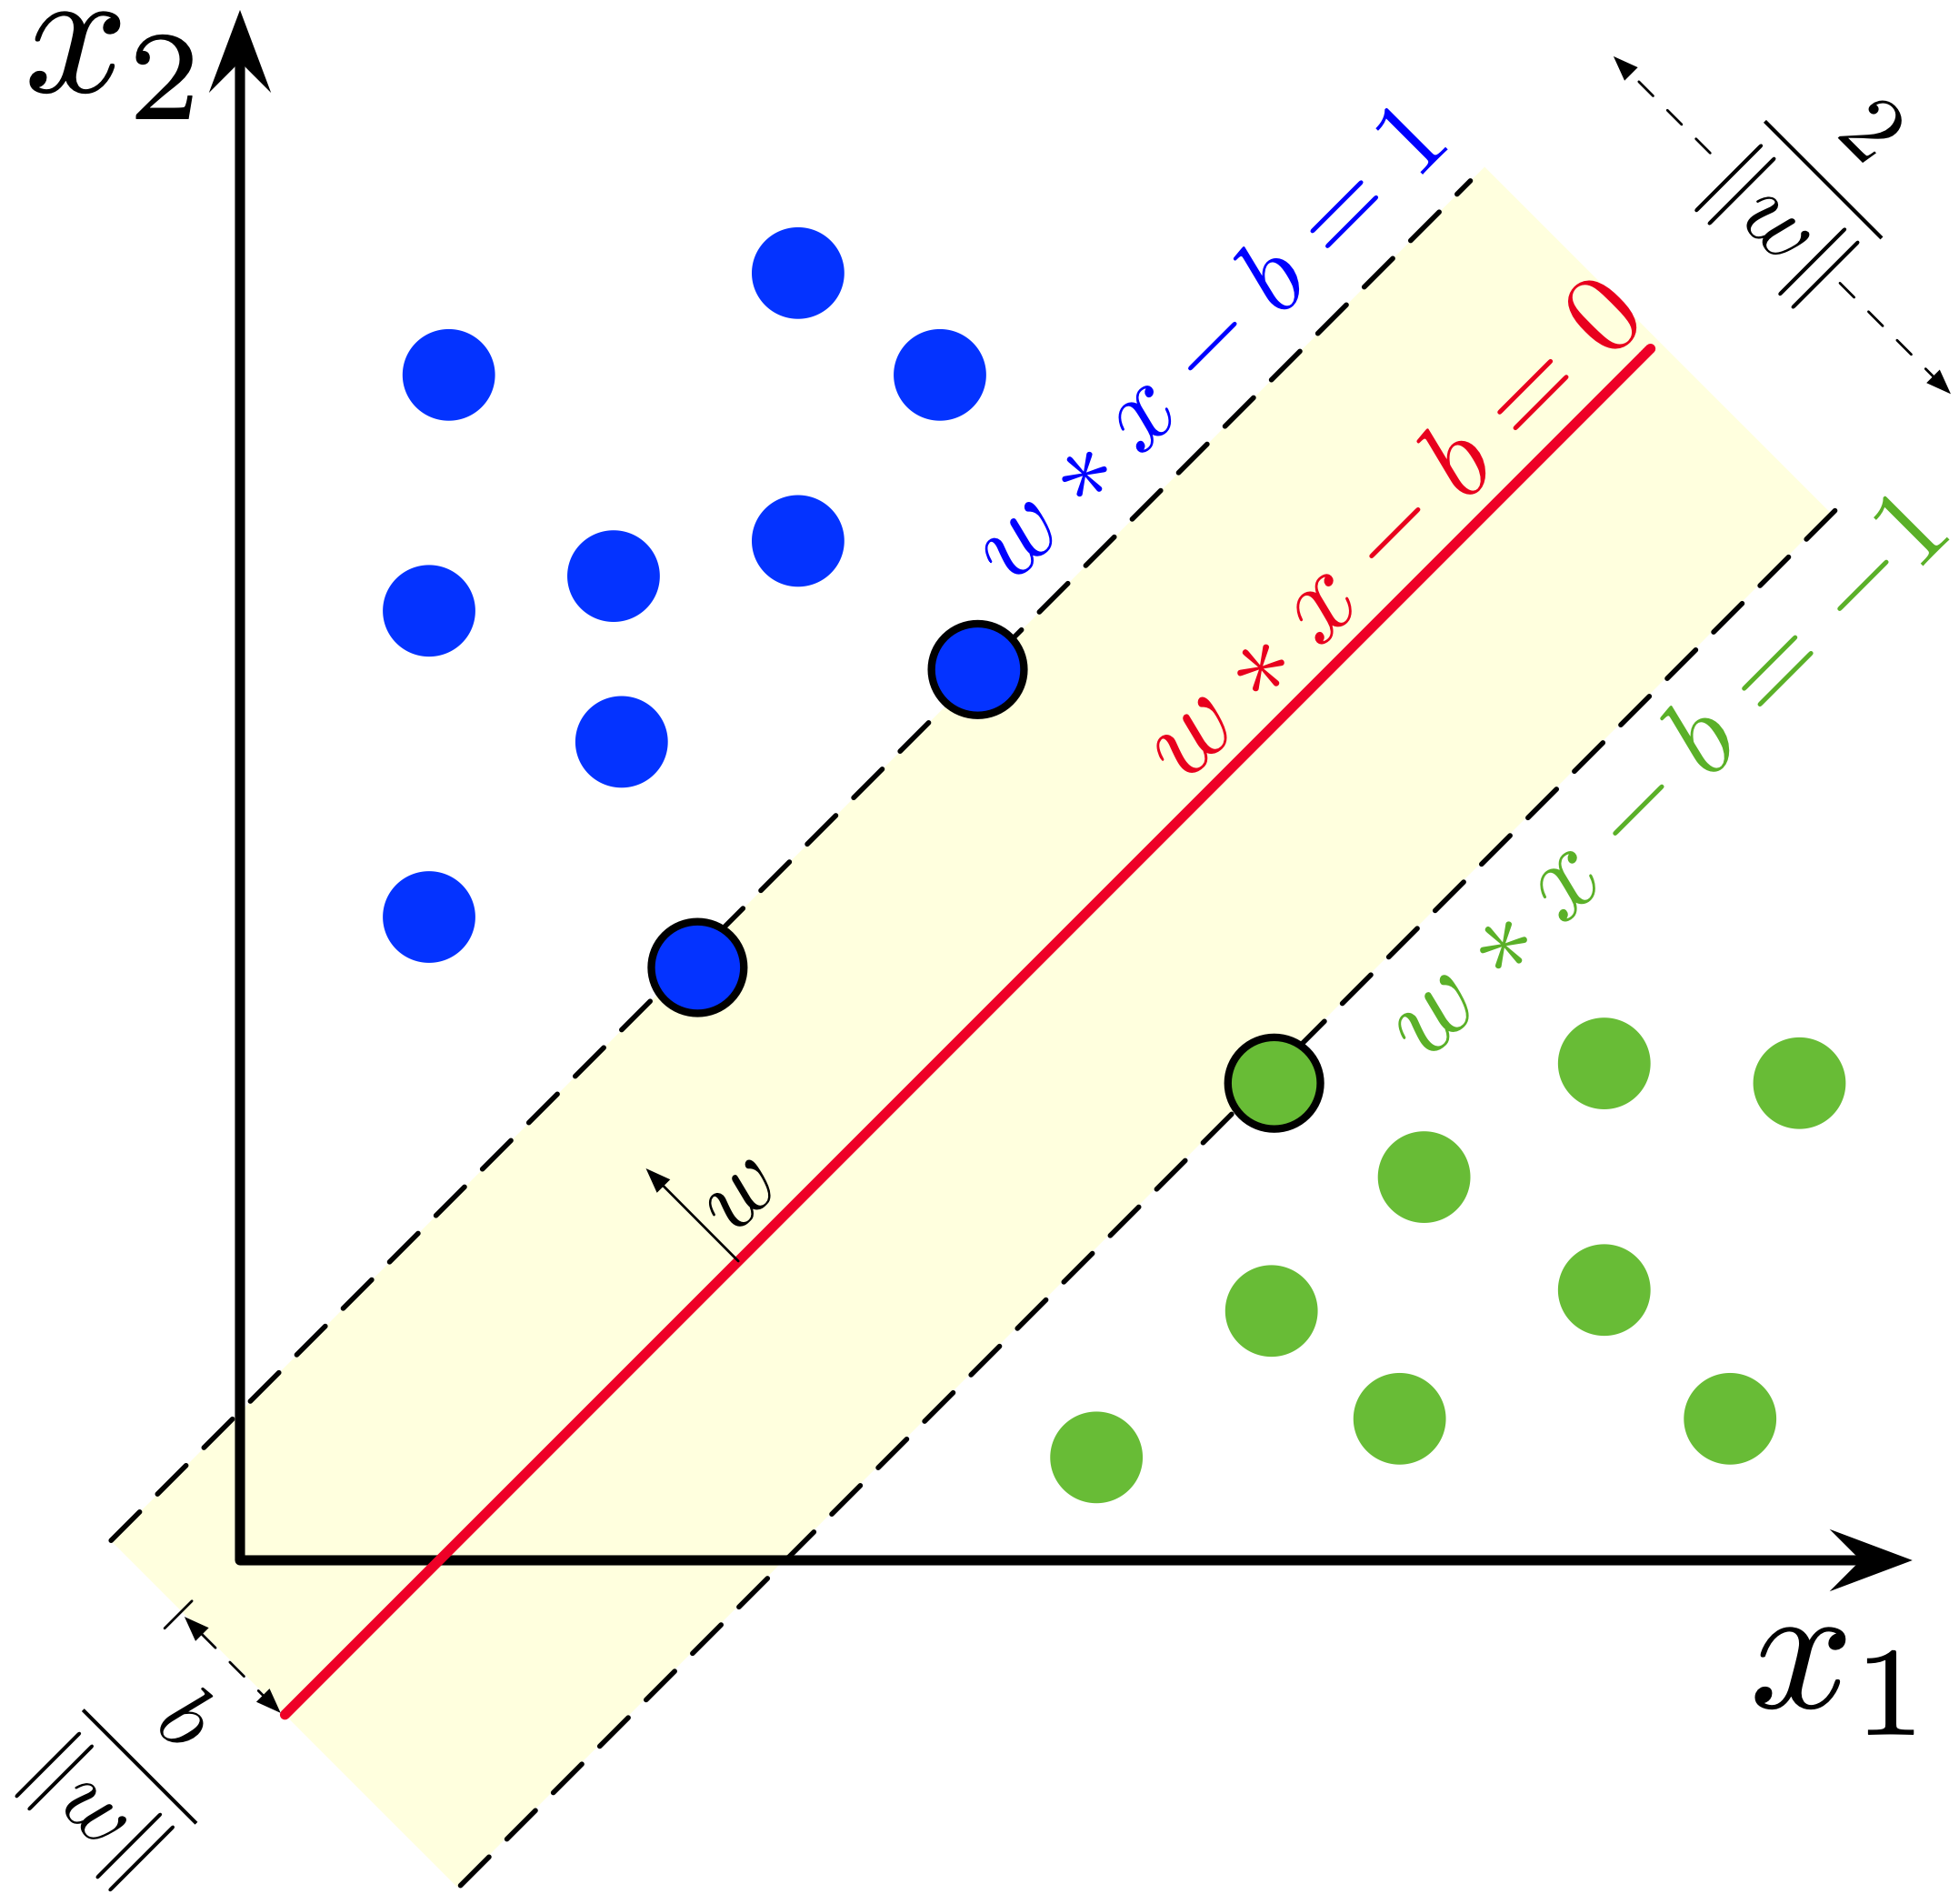
\includegraphics[height=\textheight]{FIGS_slides/SVM_margin}
    \end{minipage}
    \begin{minipage}{0.28\textwidth}
        Maximum-margin hyperplane and margins for an SVM trained with samples from two classes. Samples on the margin are the \textbf{support vectors}
    \end{minipage}
\end{frame}

\begin{frame}
    Any \textbf{hyperplane} can be written as the set of points $\mathbf{x}$ satisfying
    \[
        \bw^\mathsf{T} \bx - b = 0
    \]
    where $\bw$ is the (not necessarily normalized) \textbf{normal vector} to the hyperplane (if the hyperplane has equation $a_1z_1+\cdots+a_pz_p=c$, then $(a_1,\ldots,a_n)$ is normal to the hyperplane)
    % \vfill
    % This is much like \textbf{Hesse normal form}, except that $\mathbf{w}$ is not necessarily a unit vector
    \vfill
    The parameter $b/\|\bw\|$ determines the offset of the hyperplane from the origin along the normal vector $\bw$
    \vfill
    Remark: a hyperplane defined thusly is not a subspace of $\IR^p$ unless $b=0$. We can of course transform the data so that it is...
\end{frame}

\begin{frame}{Linearly separable points}
    Let $X_1$ and $X_2$ be two sets of points in $\IR^n$ 
    \vfill
    Then $X_1$ and $X_2$ are \textbf{linearly separable} if there exist $w_{1}, w_{2},..,w_{n}, k\in\IR$ such that 
    \begin{itemize}
        \item every point $x \in X_1$ satisfies $\sum^{n}_{i=1} w_{i}x_{i} > k$ 
        \item every point $x \in X_2$ satisfies $\sum^{n}_{i=1} w_{i}x_{i} < k$
    \end{itemize}
    where $x_{i}$ is the $i$th component of $x$
\end{frame}

\begin{frame}{Hard-margin SVM}
    If the training data is \textbf{linearly separable}, we can select two parallel hyperplanes that separate the two classes of data, so that the distance between them is as large as possible 
    \vfill
    The region bounded by these two hyperplanes is called the ``margin'', and the maximum-margin hyperplane is the hyperplane that lies halfway between them
    \vfill
    With a normalized or standardized dataset, these hyperplanes can be described by the equations
    \begin{itemize}
        \item $\mathbf{w}^\mathsf{T} \mathbf{x} - b = 1$ (anything on or above this boundary is of one class, with label 1) 
        \item $\mathbf{w}^\mathsf{T} \mathbf{x} - b = -1$ (anything on or below this boundary is of the other class, with label -1)
    \end{itemize}
\end{frame}

\begin{frame}
    Distance between these two hyperplanes is $2/\|\bw\|$
    \vfill
    $\Rightarrow$ to maximize the distance between the planes we want to minimize $\|\bw\|$
    \vfill
    The distance is computed using the distance from a point to a plane equation
    \vfill
    We must also prevent data points from falling into the margin, so we add the following constraint: for each $i$ either
    \[
        \mathbf{w}^\mathsf{T} \mathbf{x}_i - b \ge 1 \, , \text{ if } y_i = 1
    \]
    or
    \[
        \mathbf{w}^\mathsf{T} \mathbf{x}_i - b \le -1 \, , \text{ if } y_i = -1
    \]
    \vfill
    (Each data point must lie on the correct side of the margin)
\end{frame}

\begin{frame}
    This can be rewritten as
    \[
        y_i(\mathbf{w}^\mathsf{T} \mathbf{x}_i - b) \ge 1, \quad \text{ for all } 1 \le i \le n
    \]
    \vfill
    We get the optimization problem:
    \begin{quote}
        Minimize $\|\mathbf{w}\|$ subject to $y_i(\mathbf{w}^\mathsf{T} \mathbf{x}_i - b) \ge 1$ for $i = 1, \ldots, n$
    \end{quote}
    \vfill
    The $\mathbf{w}$ and $b$ that solve this problem determine our classifier, $\mathbf{x} \mapsto \sgn(\mathbf{w}^\mathsf{T} \mathbf{x} - b)$ where $\sgn(\cdot)$ is the \textbf{sign function}.
\end{frame}

\begin{frame}   
    The maximum-margin hyperplane is completely determined by those $\bx_i$ that lie nearest to it. 
    \vfill
    These $\bx_i$ are the \textbf{support vectors}
\end{frame}

\begin{frame}{Soft-margin SVM}
    To extend SVM to cases in which the data are not linearly separable, the \textbf{hinge loss} function is helpful
    \[
        \max\left(0, 1 - y_i(\mathbf{w}^\mathsf{T} \mathbf{x}_i - b)\right)
    \]
    \vfill
    $y_i$ is the $i$th target (i.e., in this case, 1 or -1), and $\mathbf{w}^\mathsf{T} \mathbf{x}_i - b$ is the $i$-th output
    \vfill
    This function is zero if the constraint is satisfied, in other words, if $\mathbf{x}_i$ lies on the correct side of the margin
    \vfill 
    For data on the wrong side of the margin, the function's value is proportional to the distance from the margin
\end{frame}

\begin{frame}
   
    The goal of the optimization then is to minimize
    
    \[ 
        \lambda \lVert \mathbf{w} \rVert^2 +\left[\frac 1 n \sum_{i=1}^n \max\left(0, 1 - y_i(\mathbf{w}^\mathsf{T} \mathbf{x}_i - b)\right) \right]
    \]
    
    where the parameter $\lambda > 0$ determines the trade-off between increasing the margin size and ensuring that the $\mathbf{x}_i$ lie on the correct side of the margin. Thus, for sufficiently small values of $\lambda$, it will behave similar to the hard-margin SVM, if the input data are linearly classifiable, but will still learn if a classification rule is viable or not
    % (This parameter $\lambda$ is often also called $C$, e.g. in ''[[LIBSVM]]'', but usually refers to the inverse of $\lambda$.)
        
\end{frame}

\end{document}